\chapter{สรีรวิทยาเฉดสีและสุขภาพธาตุอาหารพืช}

\section{สรีรวิทยาของสีใบพืชและความสัมพันธ์กับธาตุอาหาร}
สีของใบไม้ทุเรียนเป็นดัชนีชี้วัดสถานะทางสรีรวิทยาและระดับความสมบูรณ์ของธาตุอาหารโดยตรง กระบวนการสังเคราะห์แสงขับเคลื่อนด้วยรงควัตถุหลักสองชนิด คือ คลอโรฟิลล์เอ ($\text{Chlorophyll } a$) ซึ่งมีจุดดูดกลืนแสงสูงสุดที่ความยาวคลื่น $430\text{ nm}$ และ $662\text{ nm}$ และคลอโรฟิลล์บี ($\text{Chlorophyll } b$) ซึ่งมีจุดดูดกลืนแสงสูงสุดที่ $453\text{ nm}$ และ $642\text{ nm}$ ในขณะที่แถบแสงสีเขียวช่วงความยาวคลื่น $500 - 560\text{ nm}$ จะถูกสะท้อนกลับออกมาสู่สายตาและตัวรับรู้ของกล้องถ่ายภาพ

เมื่อพืชได้รับธาตุอาหารไม่สมดุล สมดุลทางชีวเคมีของการสังเคราะห์และการสลายตัวของรงควัตถุจะเปลี่ยนแปลงไปอย่างมีนัยสำคัญ ส่งผลให้เกิดการสะท้อนและการดูดกลืนแสงที่ผิดปกติไป ซึ่งสามารถวิเคราะห์แยกแยะได้ด้วยการแปลงสัญญาณภาพเข้าสู่ปริภูมิสีสากล

\section{ลายเซ็นต์ทางแสงและการเปลี่ยนแปลงเฉดสีตามชนิดธาตุอาหาร}
การตรวจประเมินภาวะขาดธาตุอาหารในระบบ DurianLeaf AI ครอบคลุมธาตุอาหารพืช 8 ชนิด โดยแต่ละธาตุมีลายเซ็นต์ทางแสง (Spectral and Colorimetric Signatures) และพิกัดสีมาตรฐานดังแสดงในตารางที่ \ref{tab:nutrient_color_profiles}

\begin{table}[h]
\centering
\caption{คุณลักษณะทางแสงและพิกัดสีมาตรฐานของภาวะโภชนาการในใบพืชทุเรียน}
\label{tab:nutrient_color_profiles}
\small
\begin{tabular}{|l|c|c|c|c|c|l|}
\hline
\textbf{ธาตุอาหาร} & \textbf{สัญลักษณ์} & \textbf{รหัสสี HEX} & $L^*$ & $a^*$ & $b^*$ & \textbf{ลักษณะอาการทางสายตาและสรีรวิทยา} \\
\hline
ปกติสมบูรณ์ & Optimal & \texttt{\#1B5E20} & 42.0 & -24.5 & 26.2 & เขียวเข้มจัด มันวาว คลอโรฟิลล์ SPAD $>48$ \\
ไนโตรเจนต่ำ & N Def & \texttt{\#FBC02D} & 76.5 & -4.8 & 62.1 & เหลืองซีดสม่ำเสมอทั่วทั้งใบ เริ่มจากใบแก่ \\
ฟอสฟอรัสต่ำ & P Def & \texttt{\#4A148C} & 24.2 & 14.8 & -8.2 & เขียวคล้ำอมม่วงแดง แอนโทไซยานินสะสม \\
โพแทสเซียมต่ำ & K Def & \texttt{\#D84315} & 45.2 & 12.6 & 28.4 & ขอบใบไหม้แห้งสีน้ำตาลทอง (Marginal Scorch) \\
แมกนีเซียมต่ำ & Mg Def & \texttt{\#C0CA33} & 68.4 & -12.4 & 48.2 & เหลืองระหว่างเส้นใบรูปก้างปลาคว่ำ \\
แคลเซียมต่ำ & Ca Def & \texttt{\#795548} & 38.6 & 6.2 & 10.4 & ปลายใบอ่อนม้วนงอ ขอบใบหงิก เนื้อเยื่อเจริญตาย \\
เหล็กต่ำ & Fe Def & \texttt{\#FFF59D} & 88.2 & -2.1 & 32.5 & ใบยอดซีดขาวเกือบทั้งใบ เส้นใบยังเขียวจาง \\
สังกะสีต่ำ & Zn Def & \texttt{\#E6EE9C} & 72.1 & -8.5 & 36.4 & โรคใบแก้ว ใบเล็กเรียวเป็นกระจุก ด่างเหลือง \\
โบรอนต่ำ & B Def & \texttt{\#8D6E63} & 42.1 & 8.4 & 14.2 & ใบหนาเปราะ เส้นใบปูดโปนเป็นตุ่มนูน \\
\hline
\end{tabular}
\end{table}

\subsection{การขาดธาตุไนโตรเจน (Nitrogen Deficiency: N)}
ไนโตรเจนเป็นองค์ประกอบโครงสร้างหลักของโมเลกุลคลอโรฟิลล์และกรดอะมิโน เมื่อเกิดภาวะขาดแคลน พืชจะสลายโปรตีนและคลอโรฟิลล์จากใบแก่ด้านล่างเพื่อลำเลียงไปยังยอดอ่อน ส่งผลให้เกิดอาการเหลืองซีดสม่ำเสมอทั่วทั้งแผ่นใบ (General Chlorosis) ค่าความสว่าง $L^*$ จะเพิ่มขึ้นอย่างมากสู่ช่วง $70 - 80$ และค่าสีเหลือง $b^*$ จะเพิ่มขึ้นสูงกว่า $55$ ในขณะที่ค่า SPAD จะลดลงต่ำกว่า $32$

\subsection{การขาดธาตุฟอสฟอรัส (Phosphorus Deficiency: P)}
ฟอสฟอรัสมีบทบาทสำคัญในการขนส่งพลังงานในรูป ATP และโครงสร้างกรดนิวคลีอิก การขาดฟอสฟอรัสทำให้การเจริญเติบโตชะงักงัน ส่งผลให้เกิดการสะสมน้ำตาลโมเลกุลเดี่ยวและกระตุ้นการสังเคราะห์สารสีกลุ่มแอนโทไซยานิน (Anthocyanin Overaccumulation) แผ่นใบแก่จะมีสีเขียวคล้ำทึบผิดปกติและปรากฏเฉดสีม่วงแดงหรือม่วงคล้ำ (\texttt{\#4A148C}) ขอบใบไหม้แห้งและค่า $a^*$ มีค่าบวกชัดเจน

\subsection{การขาดธาตุโพแทสเซียม (Potassium Deficiency: K)}
โพแทสเซียมทำหน้าที่ควบคุมแรงดันเต่ง การเปิดปิดปากใบ และการกระตุ้นเอนไซม์ เมื่อขาดโพแทสเซียม ขอบใบจะสูญเสียน้ำและคลอโรฟิลล์เสื่อมสลาย เกิดอาการขอบใบเหลืองและไหม้แห้งลามจากปลายใบเข้าสู่โคนใบเป็นสีน้ำตาลทอง (Marginal Chlorosis and Necrosis) พิกัดสีบริเวณขอบใบจะมีค่า $a^*=12.6$ และ $b^*=28.4$

\subsection{การขาดธาตุแมกนีเซียม (Magnesium Deficiency: Mg)}
แมกนีเซียมเป็นอะตอมศูนย์กลางของวงแหวนพอร์ไฟรินในโมเลกุลคลอโรฟิลล์ เนื่องจากแมกนีเซียมเป็นธาตุเคลื่อนย้ายได้ง่าย อาการขาดจะปรากฏบนใบแก่ก่อน โดยเนื้อเยื่อใบระหว่างเส้นใบหลักจะสูญเสียคลอโรฟิลล์เปลี่ยนเป็นสีเหลืองสว่าง ในขณะที่เส้นใบหลักและเส้นใบย่อยยังคงมีแถบสีเขียวเข้ม เกิดเป็นลวดลายก้างปลาคว่ำ (Inverted V-shape Chlorosis)

\subsection{การขาดจุลธาตุเหล็ก สังกะสี และโบรอน (Micronutrient Deficiencies)}
\begin{itemize}
  \item \textbf{การขาดธาตุเหล็ก (Fe)} เนื่องจากเหล็กเป็นธาตุที่เคลื่อนย้ายไม่ได้ อาการจะปรากฏบนใบอ่อนและยอดแรกผลิก่อน เนื้อเยื่อใบอ่อนจะเปลี่ยนเป็นสีขาวซีดอมเหลืองอย่างรุนแรง ($L^*>85$) ในขณะที่โครงร่างเส้นใบยังคงมีสีเขียวจางๆ ปรากฏเด่นชัด (Veinal Reticulation)
  \item \textbf{การขาดธาตุสังกะสี (Zn)} ทำให้เกิดอาการข้อปล้องสั้น แผ่นใบมีขนาดเล็กเรียว แคบ และขึ้นเป็นกระจุกคล้ายดอกกุหลาบ (Rosetting หรือ Little Leaf) เนื้อเยื่อใบด่างเหลืองเป็นหย่อม
  \item \textbf{การขาดธาตุโบรอน (B)} ส่งผลต่อการแบ่งเซลล์และผนังเซลล์ ใบแก่จะหนาด้าน กรอบ เปราะหักง่าย เส้นใบด้านล่างปูดโปนและปริแตกเป็นตุ่มสีน้ำตาล ปลายใบม้วนงอ
\end{itemize}

\subsection{ภาวะได้รับธาตุอาหารเกินเกณฑ์และความเป็นพิษ (Nutrient Excess and Toxicity)}
ภาวะธาตุอาหารเกิน โดยเฉพาะไนโตรเจนเกิน (Nitrogen Excess) ส่งผลให้เนื้อเยื่อใบเจริญเติบโตรวดเร็วเกินไป แผ่นใบมีสีเขียวเข้มคล้ำผิดปกติ แผ่นใบบิดเบี้ยวเป็นลอนหรือปลายใบงุ้มลง ผนังเซลล์บางและเปราะ อวบน้ำ ขาดความแข็งแรง ทำให้เสี่ยงต่อการถูกเชื้อราเข้าทำลายและแมลงศัตรูพืชรบกวนได้ง่าย อีกทั้งยังยับยั้งการดูดซึมธาตุแคลเซียมและโพแทสเซียม ในขณะที่ค่า SPAD จะพุ่งสูงเกิน $58.0$ และมีค่าความสว่าง $L^* < 30.0$

\begin{figure}[h]
\centering
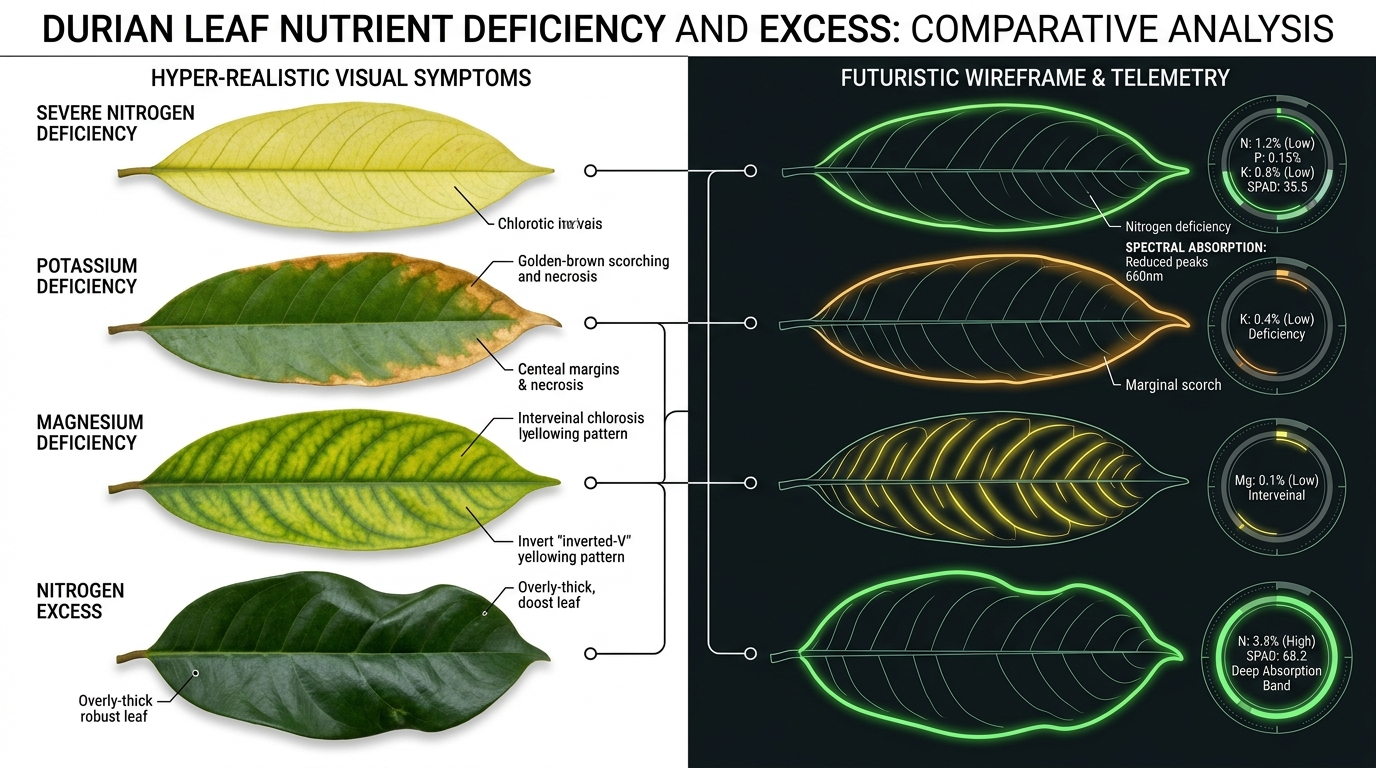
\includegraphics[width=0.96\textwidth]{figures/durian_nutrition_dual_art.jpg}
\caption{การเปรียบเทียบอาการขาดและเกินของธาตุอาหารพืชระหว่างภาพถ่ายสมจริงกับภาพโครงร่างเชิงลายเส้นและโทรมาตรปัญญาประดิษฐ์}
\label{fig:durian_nutrition_dual}
\end{figure}

รูปที่ \ref{fig:durian_nutrition_dual} แสดงการวิเคราะห์ความสมบูรณ์และโภชนาการพืชแบบคู่ขนาน (Dual-Modality Nutrition Representation) โดยฝั่งซ้ายเป็นภาพถ่ายมาโครสมจริง แสดงอาการผิดปกติทางสรีรวิทยาของใบพืช ได้แก่ ภาวะขาดไนโตรเจน (ใบเหลืองซีดสม่ำเสมอ), ภาวะขาดโพแทสเซียม (ขอบใบไหม้แห้งสีน้ำตาลทอง), ภาวะขาดแมกนีเซียม (เนื้อเยื่อระหว่างเส้นใบเหลืองเป็นรูปก้างปลาคว่ำ) และภาวะไนโตรเจนเกิน (ใบเขียวเข้มคล้ำผิดปกติและขอบบิดเบี้ยว) ในขณะที่ฝั่งขวาคือภาพเชิงลายเส้นเรืองแสง (Futuristic Vector Wireframe) พร้อมวงแหวนโทรมาตร HUD อัจฉริยะ ซึ่งจำลองการสแกนและสกัดคุณลักษณะทางแสงของปัญญาประดิษฐ์ คำนวณสัดส่วนธาตุ N, P, K, ดัชนีความเขียว SPAD และจุดพีคการดูดกลืนแสงที่ความยาวคลื่น $660\text{ nm}$ ได้ในทันที

\section{การสเปกโทรสโกปีคลอโรฟิลล์เสมือนและการคำนวณค่า SPAD}
ระบบ DurianLeaf AI ผสานข้อมูลสีเข้ากับแบบจำลองการถดถอยพหุคูณ เพื่อแปลงพิกัดสีเชิงแสงเป็นค่าดัชนีคลอโรฟิลล์ SPAD โดยปรับเทียบกับเครื่องวัดคลอโรฟิลล์มาตรฐาน Minolta SPAD-502 ดังสมการ
\begin{equation}
  \text{SPAD} = 15.20 + (52.4 \times \text{DGCI}) - (0.38 \times a^*) - 0.22 \times (L^* - 40.0) + (0.15 \times \text{GLI})
\end{equation}
โดยค่า SPAD จะถูกจัดแบ่งออกเป็น 5 ช่วงการประเมินความสมบูรณ์ ได้แก่
\begin{enumerate}
  \item $\text{SPAD} < 28$ ภาวะขาดไนโตรเจนและคลอโรฟิลล์ขั้นวิกฤต (ใบเหลืองซีด)
  \item $28 \le \text{SPAD} < 38$ ภาวะคลอโรฟิลล์ต่ำกว่าเกณฑ์ (ควรเสริมปุ๋ยไนโตรเจนและแมกนีเซียม)
  \item $38 \le \text{SPAD} < 48$ ระดับความสมบูรณ์ปานกลาง (เกณฑ์ปกติช่วงเตรียมใบ)
  \item $48 \le \text{SPAD} \le 58$ ระดับความสมบูรณ์สูงสุด (เขียวเข้ม เหมาะแก่การสะสมอาหารสร้างดอก)
  \item $\text{SPAD} > 58$ ปริมาณไนโตรเจนสูงเกินเกณฑ์ (เสี่ยงต่อการเกิดยอดแตกใบอ่อนแทนตาดอก)
\end{enumerate}

\section{สรีรวิทยาไม้ผลเมืองร้อนและแบบจำลองการประเมินธาตุอาหารเชิงปริมาณ}
การวินิจฉัยธาตุอาหารในไม้ผลยืนต้นเขตร้อนชื้น โดยเฉพาะทุเรียนพันธุ์การค้า (\textit{Durio zibethinus} L.) ไม่อาจพิจารณาจากสีของใบเพียงมิติเดียวได้ เนื่องจากความเข้มข้นของธาตุอาหารและพฤติกรรมทางสรีรวิทยาขึ้นอยู่กับตำแหน่งอายุใบและระยะพัฒนาการของทรงพุ่ม ระบบ DurianLeaf AI จึงได้บูรณาการตัวแปรทางสรีรวิทยาไม้ผลเมืองร้อน (Tropical Pomology Factors) เข้าสู่เอนจินการวิเคราะห์

\subsection{การจำแนกรุ่นใบและตำแหน่งใบ (Leaf Chronological Age Stage)}
เนื้อเยื่อใบในแต่ละช่วงอายุมีโครงสร้างทางจุลกายวิภาคและความเข้มข้นของคลอโรฟิลล์แตกต่างกันอย่างมีนัยสำคัญ ระบบแบ่งรุ่นใบออกเป็น 3 ระยะสรีรวิทยา
\begin{enumerate}
  \item \textbf{ใบอ่อน (Flush Leaf)} ใบที่เพิ่งผลิออกจากยอด อายุประมาณ $1 - 2$ สัปดาห์ สีเขียวตองอ่อนปนน้ำตาลทอง ผิวใบบางและยังสะสมไขเคลือบใบไม่สมบูรณ์ ค่าคลอโรฟิลล์ต่ำ ($\text{SPAD } 15 - 28$) ธาตุอาหารส่วนใหญ่ถูกนำเข้าจากส่วนอื่นของต้น
  \item \textbf{ใบเพสลาด (Mature Leaf)} ใบที่เจริญเติบโตเต็มที่แต่ยังไม่อาวุโส อายุประมาณ $4 - 8$ สัปดาห์ สีเขียวสดเป็นมันวาว มีอัตราการสังเคราะห์แสงสุทธิสูงสุด เป็นตำแหน่งใบอ้างอิงมาตรฐานทางวิชาการ (Standard Index Leaf) สำหรับการสุ่มตรวจประเมินโภชนาการพืช
  \item \textbf{ใบแก่ (Old Leaf)} ใบที่มีอายุมากกว่า $12$ สัปดาห์ขึ้นไป สีเขียวเข้มคล้ำ ผิวใบด้านหนา มีการสะสมสารประกอบฟีนอลและลิกนินสูง ทำหน้าที่เป็นแหล่งสะสมธาตุอาหารสำรองสำหรับการเคลื่อนย้ายกลับ
\end{enumerate}

\subsection{สรีรวิทยาการเคลื่อนย้ายธาตุอาหารในท่อน้ำท่ออาหาร (Nutrient Mobility Dynamics)}
การแสดงออกของอาการขาดธาตุอาหารบนตำแหน่งใบสัมพันธ์กับความสามารถในการเคลื่อนย้ายผ่านท่อลำเลียงอาหาร (Phloem Mobility)
\begin{itemize}
  \item \textbf{กลุ่มธาตุเคลื่อนย้ายได้สูง (Mobile Elements: N, P, K, Mg)} เมื่อเกิดภาวะขาดแคลน พืชจะสลายธาตุอาหารเหล่านี้จากใบแก่ที่อยู่ส่วนล่าง แล้วลำเลียงย้อนกลับผ่านท่อโฟลเอ็มขึ้นไปหล่อเลี้ยงยอดอ่อนและใบอ่อน ดังนั้น อาการขาดธาตุกลุ่มนี้จะปรากฏที่ \textbf{ใบแก่} ก่อนเสมอ
  \item \textbf{กลุ่มธาตุเคลื่อนย้ายยากหรือไม่เคลื่อนย้าย (Immobile Elements: Ca, Fe, Zn, B)} ธาตุกลุ่มนี้ถูกตรึงอยู่ในโครงสร้างผนังเซลล์และโมเลกุลเอนไซม์ ไม่สามารถดึงกลับมาใช้ซ้ำได้ เมื่อดินขาดธาตุอาหาร อาการผิดปกติจะปรากฏที่ \textbf{ยอดอ่อนและใบอ่อน} เป็นอันดับแรก ในขณะที่ใบแก่ยังคงมีสีเขียวปกติ
\end{itemize}

\subsection{ระยะพัฒนาการทรงพุ่มและระบบความปลอดภัยในการให้ปุ๋ย (Crop Stages and Safety Constraints)}
การจัดการธาตุอาหารในสวนทุเรียนต้องสอดคล้องกับวงจรการผลิต 5 ระยะพัฒนาการ
\begin{enumerate}
  \item \textbf{ระยะฟื้นต้นทำใบ (Vegetative Recovery)} เน้นการเสริมสร้างใบใหม่ $2 - 3$ ชุด ต้องการธาตุไนโตรเจนและแมกนีเซียมสูงเพื่อสร้างคลอโรฟิลล์
  \item \textbf{ระยะสะสมอาหารรอออกดอก (Floral Induction)} เป็นระยะวิกฤตที่ต้องการอัตราส่วนคาร์บอนต่อไนโตรเจน ($C:N\text{ Ratio}$) สูง พืชต้องลดปริมาณไนโตรเจนและสะสมฟอสฟอรัสและโพแทสเซียม
  \item \textbf{ระยะดอกบาน หางแย้ และผลอ่อน (Flowering \& Fruit Set)} ต้องการแคลเซียมและโบรอนสูงเพื่อความสมบูรณ์ของละอองเกสรและการผสมเกสร
  \item \textbf{ระยะขยายผลสร้างเนื้อ (Fruit Expansion)} ต้องการโพแทสเซียม แมกนีเซียม และไนโตรเจนปานกลาง เพื่อสร้างพูและแป้ง
  \item \textbf{ระยะบ่มหวานก่อนเก็บเกี่ยว (Maturity \& Ripening)} ควบคุมการให้น้ำและงดการให้ปุ๋ยไนโตรเจนอย่างเด็ดขาดเพื่อกระตุ้นการเปลี่ยนแป้งเป็นน้ำตาล
\end{enumerate}

\begin{theorybox}
\textbf{ระบบป้องกันความปลอดภัยของพืช (Plant Safety Constraint Protocol)}\par
ในระยะสะสมอาหารเตรียมออกดอก (Floral Induction Phase) หากระบบตรวจวิเคราะห์พบว่าใบมีระดับไนโตรเจนต่ำ ($N < 2.0\%$) ระบบ DurianLeaf AI จะทำการ \textbf{บล็อกคำแนะนำปุ๋ยไนโตรเจนโดยอัตโนมัติ} และขึ้นข้อความเตือนด้านความปลอดภัย เนื่องจากในระยะนี้ การใส่ปุ๋ยไนโตรเจนจะกระตุ้นให้ตาดอกเปลี่ยนสภาพกลายเป็นตายอดแตกใบอ่อน (Flush Aborting Flower Buds) ส่งผลให้ผลผลิตดอกร่วงเสียหายทั้งแปลง
\end{theorybox}

\subsection{การประเมินความเข้มข้นเชิงปริมาณในหน่วย มิลลิกรัมต่อกิโลกรัม (mg/kg หรือ ppm)}
เพื่อยกระดับการตรวจวิเคราะห์จากเชิงคุณภาพสู่เชิงปริมาณระดับห้องปฏิบัติการ ระบบได้ทำการแปลงสัดส่วนร้อยละของธาตุอาหารเข้าสู่หน่วยความเข้มข้นมิลลิกรัมต่อกิโลกรัมของน้ำหนักแห้ง ($\text{mg/kg}$ หรือ $\text{ppm}$) โดยอาศัยความสัมพันธ์ตามสัดส่วนเนื้อเยื่อมาตรฐาน
\begin{equation}
  C_{\text{ppm}} = C_{\%} \times 10,000 \quad (\text{สำหรับธาตุอาหารหลักและธาตุรอง})
\end{equation}
พร้อมทั้งคำนวณค่าความเชื่อมั่นทางสถิติ ($\text{Confidence } \%$) ของการทำนายจากระยะห่างทางทัศนศาสตร์เทียบกับจุดศูนย์กลางของกลุ่มตัวอย่างอ้างอิง
\begin{equation}
  \text{Confidence} = \left( 1.0 - \frac{D_{\text{Mahalanobis}}}{D_{\text{threshold}}} \right) \times 100\%
\end{equation}

\begin{theorybox}
\textbf{ความสัมพันธ์ระหว่างดัชนี DGCI กับระดับคลอโรฟิลล์เชิงพื้นที่}\par
ดัชนี Dark Green Color Index (DGCI) เป็นการรวมค่า Hue, Saturation และ Value ในปริภูมิสี HSV เข้าด้วยกัน เพื่อสะท้อนความเข้มของสีเขียวในเนื้อเยื่อใบได้อย่างเป็นเอกภาพและลดความไวต่อความเข้มแสงแวดล้อม
\begin{equation}
  \text{DGCI} = \frac{\frac{H - 60^\circ}{60^\circ} + (1 - S) + (1 - V)}{3}
\end{equation}
เมื่อค่า $H$ วัดเป็นองศา ($0^\circ - 360^\circ$), ค่า $S$ และ $V$ อยู่ในช่วง $[0, 1]$ ค่า DGCI ที่คำนวณได้จะมีค่าระหว่าง $0$ (เหลืองซีดจัด) ถึง $1$ (เขียวเข้มลึก) ซึ่งมีความสัมพันธ์แบบเส้นตรงกับปริมาณคลอโรฟิลล์ในระดับ $R^2 > 0.92$
\end{theorybox}

\begin{promptbox}
\textbf{พรอมพ์วิศวกรรมสำหรับการประเมินธาตุอาหารและดัชนีสุขภาพพืช (Prompt Eng-02)}\par
\texttt{"Act as a Precision Agriculture Scientist and Plant Physiologist. Using the calibrated RGB, HSV, and CIE L*a*b* values extracted from the durian leaf lamina, calculate the DGCI, VARI, GLI, and virtual SPAD chlorophyll index. Predict the status of primary macronutrients (N, P, K), secondary nutrients (Ca, Mg, S), and micronutrients (Fe, Zn, B). Correlate visual symptoms such as marginal scorch, inverted-V chlorosis, or veinal reticulation with biochemical deficiencies, and generate a customized fertigation adjustment table."}
\end{promptbox}
